\section{J. Pratt, Goswami - Capturability Based Analysis and Control of Legged Robots - Part 1 \cite{Koolen:2012:CAC:2344876.2344877} - 2011}
Authors: J. Pratt, Goswami\\
Year: 2012
\subsection*{Summary}
The Capture point theory is here explained for 3D-LIP model and for the 3D-LIPM model (with non zero moment of inertia)
The \textit{capturability} is updated at the end of every stance phase: there is no way to change the capturability during the swing phase.
\begin{figure}[h!]
\begin{subfigure}
  \centering
  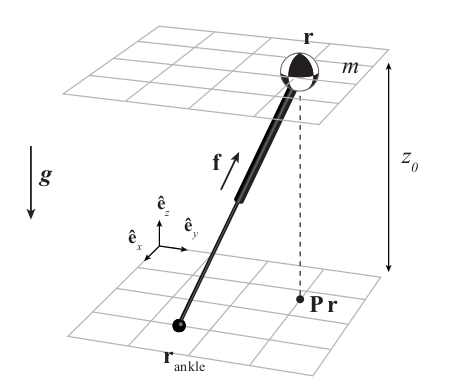
\includegraphics[width=50mm]{CP.png}
  \label{PhasePlane}
\end{subfigure}
\begin{subfigure}
  \centering
  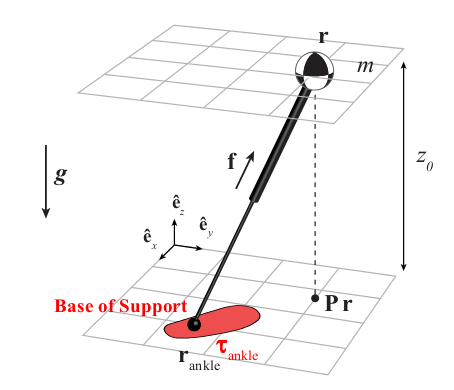
\includegraphics[width=50mm]{CPF.png}
  \label{PhasePlane}
\end{subfigure}
\begin{subfigure}
  \centering
  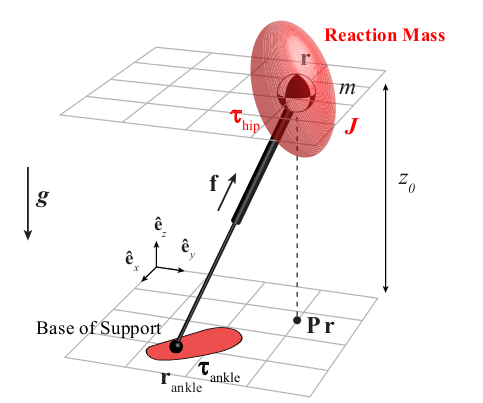
\includegraphics[width=50mm]{CPFM.png}
  \label{PhasePlane}
\end{subfigure}
\caption{three simplified models of a the dynamics of an antropomorphic robot}
\end{figure}
\begin{multicols}{3}
3D-LIP model:
\begin{enumerate}
\item Equations of motion:
$$ m \ddot{r} = mg + f $$
$$ -(r-r_{ankle})  \times f = 0 $$
\item CP definition:  $$ r_{ic} = P r + \frac{\dot{r}}{\omega} $$
\item Instantaneous CP dynamics: $$ \ddot{r} = \omega^2 (P r - r_{ankle}) $$
\item 0-step capturability:
$$ | r'_{ic} - r'_{ankle}| \le d'_0 = 0 $$
\item n-steps capturability:
$$ | r'_{ic} - r'_{ankle}| \le d'_n $$ where: $$ d'_n = (l'_{max} + d'_{n-1})e^{- \Delta t'_s}$$
\end{enumerate}
\columnbreak
3D-LIP + finite foot:
\begin{enumerate}
\item Equations of motion:
$$ m \ddot{r} = mg + f $$
$$ -(r-r_{ankle})  \times f + \tau_{ankle}= 0 $$
\item CP definition: \\
no c.f. sol.
\item Instantaneous CP dynamics:
$$ \ddot{r} = \omega^2 (P r - r_{CoP}) $$
\item 0-step capturability:
$$ | r'_{ic} - r'_{ankle}| \le d'_0 =  r'_{max} $$
\item n-steps capturability:
$$ | r'_{ic} - r'_{ankle}| \le d'_n $$ where: $ d'_n = r'_{max} + (l'_{max} - r'_{max} + d'_{n-1})e^{- \Delta t'_s}$
\end{enumerate}

\columnbreak
3D-LIP + finite foot + reaction mass:
\begin{enumerate}
\item Equations of motion:
$$ m \ddot{r} = mg + f $$
$$ J \dot{\omega} = \tau_{hip} - \omega \times (J \omega) $$
$$ -(r-r_{ankle})  \times f + \tau_{ankle} - \tau_{hip}= 0 $$
\item CP definition: 
no c.f. sol.
\item Instantaneous CP dynamics: $$ \ddot{r} = \omega^2 (P r - r_{CMP}) $$
$$ \dot{\omega} = J^{-1} P \tau_{hip} $$
\item 0-step capturability:
$$ | r'_{ic} - r'_{ankle}| \le d'_0 = r'_{max} + |\Delta r'_{CMP}|_{max}$$
\item n-steps capturability:
$$ | r'_{ic} - r'_{ankle}| \le d'_n $$ where: $ d'_n = r'_{max} + |\Delta r'_{CMP}|_{max} + (l'_{max} - r'_{max} + d'_{n-1})e^{- \Delta t'_s}$
\end{enumerate}
\end{multicols}
where:
\begin{itemize}
\item $P$ is the matrix which projects the CoM on the ground.
\item $r_{max}$ = distance between the CoP and the point on the edge of the support which is closest to the istantaneous CP.
\item CMP = Centroidal Moment Pivot point
\item $d_{\infty}$ = distance to the $\infty$-steps capturability region. This can be used as a \textbf{capturability margin}, in the sense that if the $d_{\infty}$ takes on a small value, the robot will likely fall when subject to an external disturbance. For example, using the same common parameters it was obtained that for:
\begin{itemize}
\item 3D-LIP model: $d_{\infty} = 0.431$
\item 3D-LIP model + finite foot: $d_{\infty} = 0.631$
\item 3D-LIP model + finite foot + reaction mass: $d_{\infty} = 0.664$
\end{itemize}
So we can conclude that the third model has got the \textit{highest level of capturability}, i.e. it is the most stable (see figure \ref{InftyCap}).
\\
\begin{figure}
  \centering
  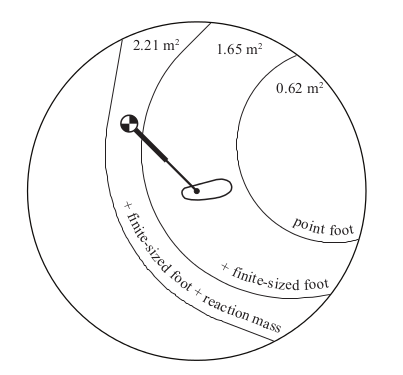
\includegraphics[width=50mm]{InftyCapturability.png}
  \caption{Comparison of the infinity-capturability distance $d_{\infty}$ for the three different considered models}
  \label{InftyCap}
\end{figure}
\end{itemize}
\subsection*{Key points / Takeaways}
\begin{itemize}
\item \textbf{Equivalent constant CoP} =
\end{itemize}
\subsection*{Weak points}
\subsection*{Ideas}

